Система будет представлять собой единый продукт, состоящий из веб-портала и серверной частей. Серверная часть отдает по интернет сети документы страниц веб-портала. Веб-портал отображает гостю новостные подборки на основной публичной странице. Так же веб-портал будет имееть страницы защищенные с помощью авторизации: страница с панелью администратора для управления сайтом и страница редактора/автора для созадания и радактирования новостных материалов. 

Для хранения новостных материалов и данных авторизованных пользователей будет использоваться хранилище информации в виде отдельной базы данных, с которой сервер будет иметь соединение. Все операции над данными в базе, инициированные с помощью веб-портала, будут выполняться с участием этого сервера.

Блочная диаграмма компонентов системы изображена на схеме \ref{fig:product-perspective}.
% [ПЕРСПЕКТИВЫ РАЗВИТИЯ СИСТЕМЫ, ИЗ КАКИХ КОМПОНЕНТОВ ПРИ ЭТОМ СОСТОИТ СИСТЕМА И КАКИЕ ИНТЕРФЕЙСЫ И АПИ ДОЛЖНЫ ПРИСУТСТВОВАТЬ]\\[5mm]
% \\ \textit{[ПОДСЕКЦИИ: \\
%     САЙТКИ МАЛЕНЬКИЙ И ВРЯД-ЛИ БУДЕТ РАЗВИВАТЬСЯ СИЛЬНО, ТАК ЧТО МОЖНО ОПУСТИТЬ ПУНКТЫ
%     % System interfaces,
%     % User intefaces,
%     % Hardware interfaces,
%     % Software interfaces,
%     % Communications interfaces,
%     % Метогу constraints,
%     % 0perations,
%     % Site adaptation requirements
% ]}

\begin{figure}[H]
    \centering
    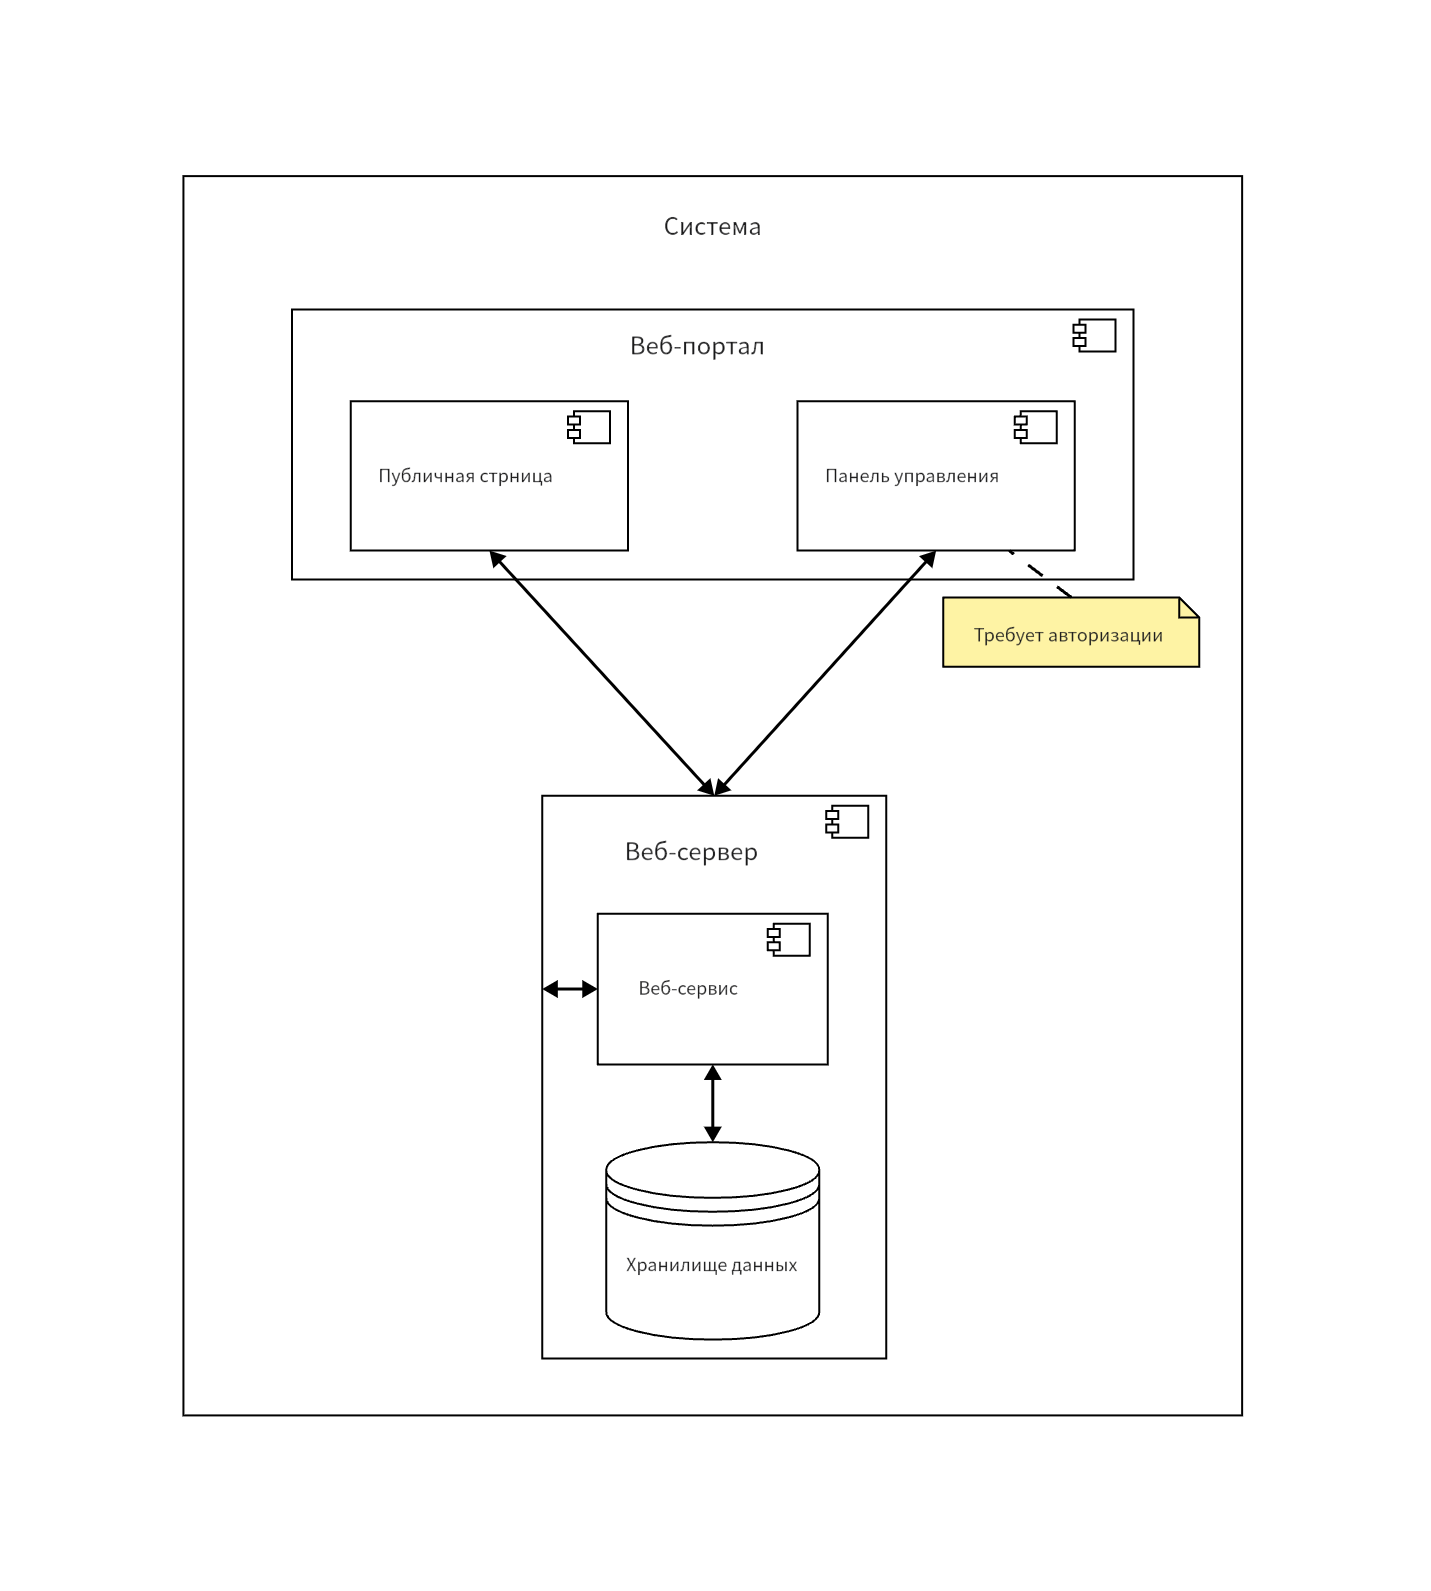
\includegraphics[width=\textwidth]{res/product-perspective.png}
    \caption{Блочная диаграмма компонентов системы}
    \label{fig:product-perspective}
\end{figure}

%%%%
% This subsection of the SRS should put the product into __perspective 
% with other__ related products. If the product is independent and 
% totally self-contained, __it shou1d be so stated here__. 
%
% If the SRS defines а product that is а component of а larger system, 
% as frequently then this subsection should relate the requirements of 
% that larger system to functionality of the software and should identify 
% interfaces between that system and the software.
%
% А __blосК diagram__ showing the major of the larger system, 
% interconnections, and external interfaces сап be helpful.
%
% This subsection should also describe how the software operates
% inside various constraints. For example, these could include:
%   а) System interfaces
%   Ь) User interfaces
%   с) Hardware interfaces
%   d) Software interfaces
%   е) Communications interfaces
%   f) Меmorу constraints
%   д) Operations
%   h) Site adaptation requirements
%